\chapter{Ergebnisse}
\label{chap:results}

\section{Diagramme}

Dies ist ein Diagramm, das mit Python (Jupyter Notebook) erstellt wurde, um den Stil des Dokuments beizubehalten.

\begin{figure}[htbp]
    \centering
    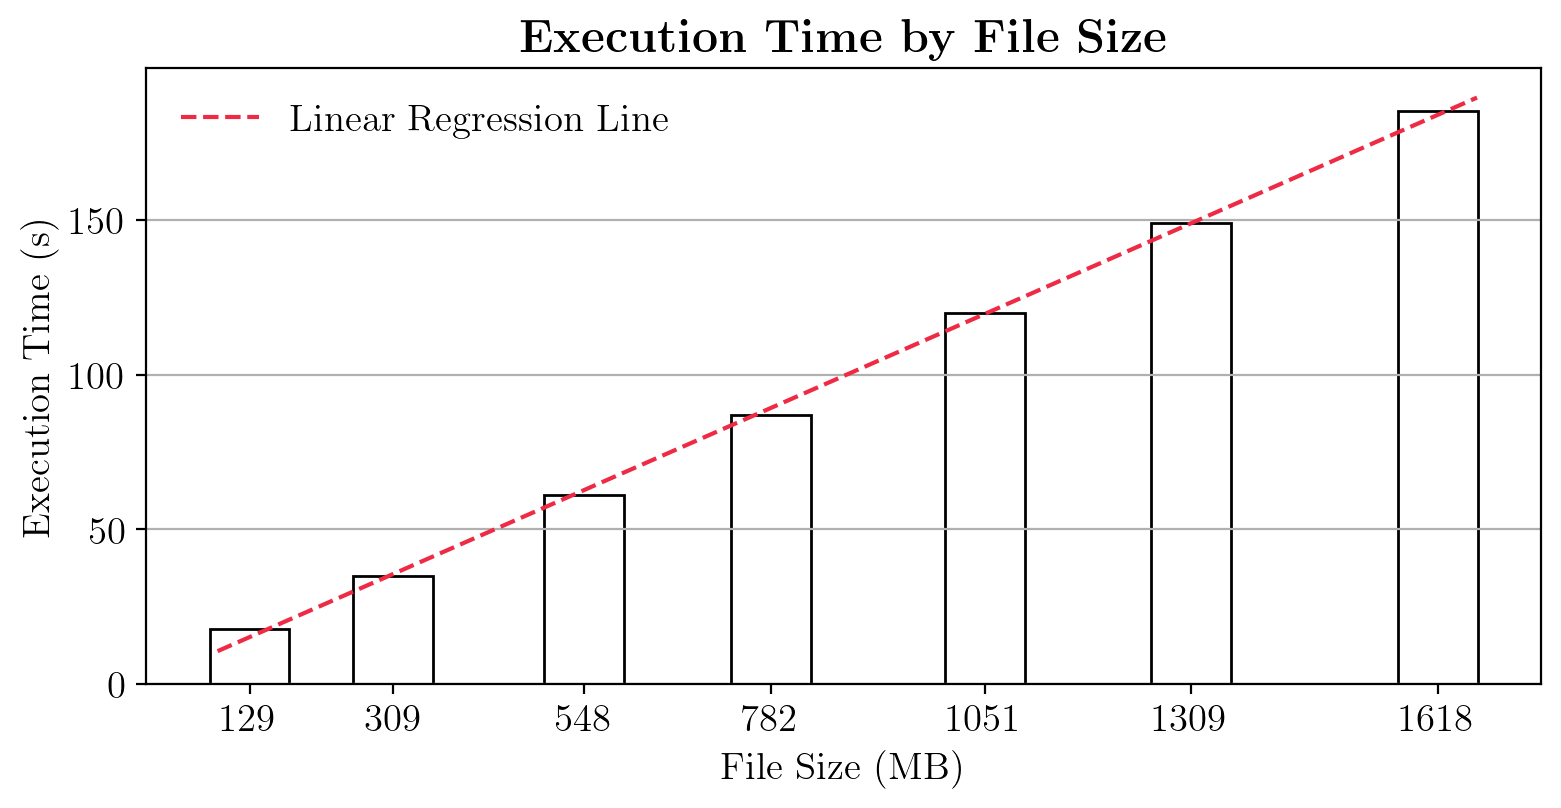
\includegraphics[width=0.9\textwidth]{figures/execution-time.png}
    \caption{Ausführungszeit nach Größe der Trace-Datei des Frameworks.}
    \label{fig:execution-time}
\end{figure}
